\documentclass{elsarticle}

%\usepackage{lineno,hyperref}
%\modulolinenumbers[5]


%%%%%%%%%%%%%%%%%%%%%%%
%% Elsevier bibliography styles
%%%%%%%%%%%%%%%%%%%%%%%
%% To change the style, put a % in front of the second line of the current style and
%% remove the % from the second line of the style you would like to use.
%%%%%%%%%%%%%%%%%%%%%%%

%% Numbered
%\bibliographystyle{model1-num-names}

%% Numbered without titles
%\bibliographystyle{model1a-num-names}

%% Harvard
%\bibliographystyle{model2-names.bst}\biboptions{authoryear}

%% Vancouver numbered
%\usepackage{numcompress}\bibliographystyle{model3-num-names}

%% Vancouver name/year
\usepackage{numcompress}\bibliographystyle{model4-names}
\usepackage{textcomp}
\usepackage{amsmath}
\usepackage{mathtools}
\DeclarePairedDelimiter\ceil{\lceil}{\rceil}
\DeclarePairedDelimiter\floor{\lfloor}{\rfloor}
\biboptions{authoryear}
\usepackage{tikz}
\usetikzlibrary{arrows.meta,chains,%
	decorations.pathreplacing}


%% APA style
%\bibliographystyle{model5-names}\biboptions{authoryear}

% AMA style
%\usepackage{numcompress}\bibliographystyle{model6-num-names}

%% `Elsevier LaTeX' style
%\bibliographystyle{elsarticle-num}
%%%%%%%%%%%%%%%%%%%%%%%

\begin{document}

\begin{frontmatter}

\title{Vendor Managed Inventory Problem for Blood Platelets: a Two Stage Deep Reinforcement Learning Approach}

\author[1]{Andres F. Osorio}
\author[2]{Juan D. Carvajal}


\address[1]{afosorio@icesi.edu.co}
\address[2]{juan030698@hotmail.com}


\begin{abstract}
	This paper presents an application of Deep Reinforcement techniques 
\end{abstract}


\end{frontmatter}

%\linenumbers

\section{Introduction}

\section{Literature Review}

\section{Problem Definition}

	\subsection{Context}
		In general terms, the supply chain of human blood products its very complicated. Blood products, specially platelets, have very short expiration periods (around 5 days). Because of this, blood managing entities , like donor centers, face great issues estimating and planning production of these vital products. These issues can be of two types, the first one, its about expiration levels, if the donor center produces too much platelets (overestimating the demand), these limited and costly to produce items will go to waste, generating high costs for the entity, and providing no benefit to final users.The second kind of issue, is related to product stock outs (underestimating the demand).Its clear that stock outs are a much more important problem for the donor centers, because these can result in increased risk of death for those needing the platelets.The gravity of this problems is only increased when multiple hospitals or medical centers, with different demand distributions are dependent on the supplies from the donor center.The basic decision for a donor center consists of two parts, the first one, its about how much to produce. Human blood can be transformed and separated into its basic constituents (platelets among these)using a process called blood fractionation,usually performed centrifuging the blood.This process is carried out using specially designed blood bags,which can be single, double, triple or quadruple.Only the last two (the most expensive ones) can be used to extract platelets, so the donor center must know how many of these bags to use in the total donor pool.The second problem its about how much to deliver to each medical center, given its demand distribution and the current inventory of the donor center.
		This problem is essentially a particular case of a Vendor Managed Inventory System, where a distribution center has to supply each of its customers based on individual needs and current capacity.
		\subsection{Modeling}
		To model such a system,a 4 medical center distribution has been considered, but the model should be easily scaled to an arbitrary number of medical centers.The medical centers will be referred from know on as hospitals.
		Each hospital has an internal inventory, visible to the donor center, this inventory is represented by a 5-tuple:
		\def\layersep{2.5cm}
		
		\begin{tikzpicture}[shorten >=1pt,->,draw=black!50, node distance=\layersep]
		\tikzstyle{every pin edge}=[<-,shorten <=1pt]
		\tikzstyle{neuron}=[circle,fill=black!25,minimum size=17pt,inner sep=0pt]
		\tikzstyle{input neuron}=[neuron, fill=green!50];
		\tikzstyle{output neuron}=[neuron, fill=red!50];
		\tikzstyle{hidden neuron}=[neuron, fill=blue!50];
		\tikzstyle{annot} = [text width=4em, text centered]
		
		% Draw the input layer nodes
		\foreach \name / \y in {1,...,4}
		% This is the same as writing \foreach \name / \y in {1/1,2/2,3/3,4/4}
		\node[input neuron, pin=left:Input \#\y] (I-\name) at (0,-\y) {};
		
		% Draw the hidden layer nodes
		\foreach \name / \y in {1,...,5}
		\path[yshift=0.5cm]
		node[hidden neuron] (H-\name) at (\layersep,-\y cm) {};
		
		% Draw the output layer node
		\node[output neuron,pin={[pin edge={->}]right:Output}, right of=H-3] (O) {};
		
		% Connect every node in the input layer with every node in the
		% hidden layer.
		\foreach \source in {1,...,4}
		\foreach \dest in {1,...,5}
		\path (I-\source) edge (H-\dest);
		
		% Connect every node in the hidden layer with the output layer
		\foreach \source in {1,...,5}
		\path (H-\source) edge (O);
		
		% Annotate the layers
		\node[annot,above of=H-1, node distance=1cm] (hl) {Hidden layer};
		\node[annot,left of=hl] {Input layer};
		\node[annot,right of=hl] {Output layer};
		\end{tikzpicture}
		
		
		
		
		

\section{Methodology}

	\subsection{Vendor Managed Inventory}

	Opposing to the traditional vendor-client systems, Vendor managed inventory systems design the supply chain architecture from the supplier to the customers.Clients must provide relevant information like inventories and sales, and is the responsibility of the vendor to define the size and date of the shipments. These systems often come with a tight information system coupling between clients and vendors, so the information is always readily available. The VMI model is going to be leveraged in order to reduce the general levels of stock-outs and expired product in the blood supply chain, more specifically the platelets supply chain.
		
	\subsection{Deep Reinforcement Learning Framework}
	
	To leverage the VMI model, the blood distribution centers (the vendors for this specific case), need a way to define optimal or near optimal policies to make shipments to the customers(hospitals and medical facilities in need of platelets).Considering that in real-world systems, demand is stochastic and often seasonal, most classic inventory policies can't be used. Also, for this specific case, the vendor does not have unlimited production capacity, because raw materials for blood products come from a variable pool of donors. Because of this,the best approach to find the shipping policies are heuristics. The chosen method to generate such policies is Deep Reinforcement Learning.This framework is based on a reward system across various simulations of the actual system, that must be represented in a way the deep learning framework can understand.
	
	\subsubsection{Data Representation}
	Typical deep reinforcement systems are modeled as a set of states and a set of actions. A state correspond to a tuple of numbers that represent certain characteristics of the system at a given time. Similarly, the action space of a system can be represented as a tuple, where each element maps directly to a well defined action. Both state and action spaces can be discrete or continuous.For this specific case, both are discrete.
	The case study system state is represented by a 10-tuple, each position of the tuple represents a characteristic of the system in the following form:
	

	\begin{center}
	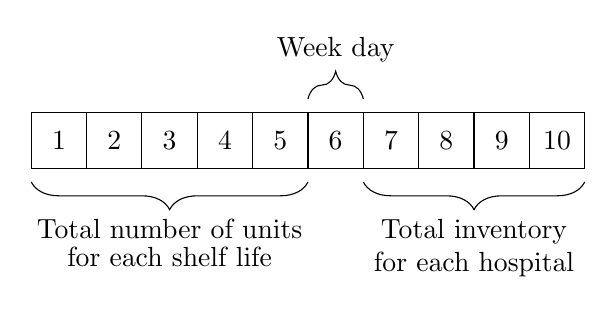
\begin{tikzpicture}[
	% -{Stealth[length = 2.5pt]},
	start chain = going right,
	node distance = 0pt,
	MyStyle/.style={draw, minimum width=2em, minimum height=2em, 
		outer sep=0pt, on chain},
	]
	\node [MyStyle] (1) {$1$};
	\node [MyStyle] (2) {$2$};
	\node [MyStyle] (3) {$3$};
	\node [MyStyle] (4) {$4$};
	\node [MyStyle] (5) {$5$};
	\node [MyStyle] (6) {$6$};
	\node [MyStyle] (7) {$7$};
	\node [MyStyle] (8) {$8$};
	\node [MyStyle] (9) {$9$};
	\node [MyStyle] (10) {$10$};

	\draw[decorate,decoration={brace, amplitude=10pt, raise=5pt, mirror}]
	(1.south west) to node[black,midway,below= 15pt] {
		\shortstack{Total number of units\\for each shelf life }} (5.south east);%
	
		\draw[decorate,decoration={brace, amplitude=10pt, raise=25pt, }]
	(6.south west) to node[black,midway,above=35pt] {Week day} (6.south east);%
	
			\draw[decorate,decoration={brace, amplitude=10pt, raise=5pt, mirror}]
	(7.south west) to node[black,midway,below= 15pt] {\shortstack{Total inventory\\for each hospital}} (10.south east);%
	
	\end{tikzpicture}
	\end{center}
	
		Position 1 to 5:
	Total number of platelets from 0 to 4 remaining days of shelf life. Items with 0 days of shelf life will expire in the current time step. Items with 4 days of remaining shelf life have just been produced.
	
	Position 6:
	Represent the day of the week from 1 to 7, Monday is the first day of the week.
	
	Position 7 to 10:
	Represent the sum of the inventory for each of the 4 hospitals connected to this vendor.
	
	Now it's clear that the state space for this system is discrete.
	
	For the action space, the scheme is very similar, the deep reinforcement agent works with discrete actions represented by a tuple.The proposed system has the need to produce two types of actions simultaneously , so we have the need to encode these two values within a single index of the action vector.
	The first type of action has to do with how many units of platelets are extracted from the collected blood for the next time step. This action can be expressed as a percentage of the total donor pool for the current time step (day).Because these percentage is a continuous quantity, we chose to discretize it into 10\% intervals,this means we have 11 values from 0\% to 100\%.
	The second kind of action is related to how much product to ship to the hospitals and medical centers (as a total). Considering the demand distribution for all the hospitals, we chose a value of 99 as an absolute maximum for this number, this means we have 100 possible values for this kind of action (from 0 to 99). If we multiply the possibilities of the two types of actions (11 x 100), we get a total of 1100 possible actions for this system. Here we can note that the action space for this system is discrete, because the system can perform one and only one action in a given time step, and the chosen action is well defined as a binary option.This means that a typical decision for this agent is a one-hot encoded vector, where the index of the one is the value for the action. This is important, because other variations of deep reinforcement learning allow the decision to be continuous, this means the agent could choose to execute several actions with values between 0 and 1.The resulting vector can be represented as follows:
	
		\begin{center}
		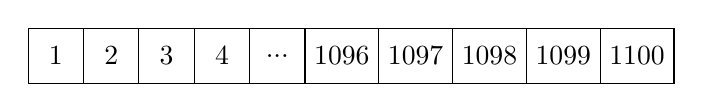
\begin{tikzpicture}[
		% -{Stealth[length = 2.5pt]},
		start chain = going right,
		node distance = 0pt,
		MyStyle/.style={draw, minimum width=2em, minimum height=2em, 
			outer sep=0pt, on chain},
		]
		\node [MyStyle] (1) {$1$};
		\node [MyStyle] (2) {$2$};
		\node [MyStyle] (3) {$3$};
		\node [MyStyle] (4) {$4$};
		\node [MyStyle] (5) {$...$};
		\node [MyStyle] (6) {$1096$};
		\node [MyStyle] (7) {$1097$};
		\node [MyStyle] (8) {$1098$};
		\node [MyStyle] (9) {$1099$};
		\node [MyStyle] (10) {$1100$};
		
		
		\end{tikzpicture}
	\end{center}

	To extract both actions based on the index of the vector, these basic operation can be performed:
	\[ Production\ \% = 10({{(n-1)}\mod11}) \]
	\[ Total\ Shipment = \floor{\frac{n-1}{11}}\]
	

	\subsection{Goal Programming Model}


\begin{equation}
	\begin{array}{ll@{}ll}
	& \displaystyle Q(s_{t},a_{t}) \longleftarrow (1 - \alpha ).Q(s_{t},a_{t}) + \alpha .(r_{t} + \gamma . \max Q(s_{t+1},a))\\
	\end{array}
	\label{eq:Eq32}
	\end{equation}	
		



\subsection{Integer Programming Model}

		
	\textbf{Objective Function}
	\begin{equation}
	\begin{array}{ll@{}ll}
	\min & \displaystyle\sum\limits_{h \in H}&(I_{h0}CV + F_{h}CF)\\
	\end{array}
	\label{eq:Eq31}
	\end{equation}

	\textbf{Constraints}
	
	\begin{equation}
	\begin{array}{ll@{}ll}
	& \displaystyle I_{h0} = \max(0, I_{h1} + X_{h1} - D_{h})\\
	\end{array}
	\label{eq:Eq32}
	\end{equation}	
		
	\begin{equation}
	\begin{array}{ll@{}ll}
	& \displaystyle F_{h} = \max(0, D_{h} - &\sum\limits_{r \in R}(I_{hr} + X_{hr}))\\
	\end{array}
	\label{eq:Eq33}	
	\end{equation}
	
	\begin{equation}
	\begin{array}{ll@{}ll}
	& \displaystyle F_{h} \leq \frac{1}{\| H \|} &\sum\limits_{h \in H}(F_{h})\\
	\end{array}
	\label{eq:Eq33}	
	\end{equation}
	
	\begin{equation}
	\begin{array}{ll@{}ll}
	& \displaystyle A_{r} = \sum\limits_{h \in H}(X_{hr})\\
	\end{array}
	\label{eq:Eq33}	
	\end{equation}

	\begin{equation}
	\begin{array}{ll@{}ll}
	& \displaystyle \frac{\sum\limits_{r \in R}(I_{hr}+X_{hr})}{D_{h}} = \frac {\sum\limits_{r \in R}(I_{h+1r}+X_{h+1r})}{D_{h+1}} \ \ \forall h<4 \\
	\end{array}
	\label{eq:Eq33}	
	\end{equation}

Constraints 2 and 3 can be linearised as follows:
 

Linearisation Equation 2
 	\begin{equation}
	\begin{array}{ll@{}ll}
	& \displaystyle -I_{h1} - X_{h1} + D_{h} \leq M*YI_{h0} \ \ \forall \ \ h\\
	\end{array}
	\label{eq:Eq33}	
	\end{equation}


 	\begin{equation}
	\begin{array}{ll@{}ll}
	& \displaystyle I_{h1} + X_{h1} - D_{h} \leq M(1-YI_{h0}) \ \ \forall \ \ h\\
	\end{array}
	\label{eq:Eq33}	
	\end{equation}

 	\begin{equation}
	\begin{array}{ll@{}ll}
	& \displaystyle I_{h0} \geq 0 \ \ \forall \ \ h\\
	\end{array}
	\label{eq:Eq33}	
	\end{equation}


 	\begin{equation}
	\begin{array}{ll@{}ll}
	& \displaystyle I_{h0} \geq I_{h1} + X_{h1} - D_{h} \ \ \forall \ \ h\\
	\end{array}
	\label{eq:Eq33}	
	\end{equation}

 	\begin{equation}
	\begin{array}{ll@{}ll}
	& \displaystyle I_{h0} \leq M(1-YI_{h0}) \ \ \forall \ \ h\\
	\end{array}
	\label{eq:Eq33}	
	\end{equation}

	\begin{equation}
	\begin{array}{ll@{}ll}
	& \displaystyle I_{h0} \leq I_{h1} + X_{h1} - D_{h} +M*YI_{h0} \ \ \forall h\\
	\end{array}
	\label{eq:Eq32}
	\end{equation}	
	
	
Linearisation Equation 3
	
	\begin{equation}
	\begin{array}{ll@{}ll}
	& \displaystyle - D_{h} + \sum\limits_{r \in R}(I_{hr} + X_{hr}) \leq M*YF_{h} \ \ \forall h\\
	\end{array}
	\label{eq:Eq32}
	\end{equation}	
	
	\begin{equation}
	\begin{array}{ll@{}ll}
	& \displaystyle D_{h} - \sum\limits_{r \in R}(I_{hr} + X_{hr}) \leq M*(1-YF_{h}) \ \ \forall h\\
	\end{array}
	\label{eq:Eq32}
	\end{equation}	
	
	 	\begin{equation}
	\begin{array}{ll@{}ll}
	& \displaystyle F_{h} \geq 0 \ \ \forall \ \ h\\
	\end{array}
	\label{eq:Eq33}	
	\end{equation}


 	\begin{equation}
	\begin{array}{ll@{}ll}
	& \displaystyle F_{h} \geq D_{h} - \sum\limits_{r \in R}(I_{hr} + X_{hr}) \ \ \forall \ \ h\\
	\end{array}
	\label{eq:Eq33}	
	\end{equation}

	
		\begin{equation}
	\begin{array}{ll@{}ll}
	& \displaystyle F_{h} \leq M(1-YF_{h}) \ \ \forall \ \ h\\
	\end{array}
	\label{eq:Eq33}	
	\end{equation}

	\begin{equation}
	\begin{array}{ll@{}ll}
	& \displaystyle F_{h} \leq D_{h} - \sum\limits_{r \in R}(I_{hr} + X_{hr}) +M*YF_{h} \ \ \forall h\\
	\end{array}
	\label{eq:Eq32}
	\end{equation}	
	
Once the model has been run, the inventory in each hospital is updated as follows:

	\begin{equation}
	\begin{array}{ll@{}ll}
	& \displaystyle I_{hr} = \max(0, I_{hr+1} + X_{h} - \max(0,D_{h}- \sum\limits_{r \in R}(I_{hr} + X_{hr}))) \ \ \forall h, \ r \neq 0 , 4 \\
	\end{array}
	\label{eq:Eq32}
	\end{equation}	

	
	\begin{equation}
	\begin{array}{ll@{}ll}
	& \displaystyle I_{h4} = \max(0, X_{4} - \max(0,D_{h}- \sum\limits_{r \in R}(I_{hr} + X_{hr})))\\
	\end{array}
	\label{eq:Eq32}
	\end{equation}	

\section{Case study}

\section{Results}

\bibliography{mybibfile}

\end{document}